% !TeX spellcheck = en_GB
\def\ChapterTitle{Modelling and Analysis of Collaborative Node Kinematic Behaviours in Underwater Acoustic \gls{manet}s}

\ifx\ifthesis\undefined
\documentclass[a4paper, 11pt]{article}

% % Special Includes stolen from Thesis.cls
\usepackage{booktabs}
\usepackage{hyperref}
\usepackage{graphicx}
\usepackage{epstopdf}
\usepackage{subcaption}
\usepackage{rotating}
\usepackage{listings}
\usepackage{lstpatch}
\renewcommand{\arraystretch}{1.3}

% % % % % % % % % % % % % % % %

% PACKAGES
\usepackage[square, numbers, comma, sort&compress]{natbib}  % Use the "Natbib" style for the references in the Bibliography
\usepackage{verbatim,listings}  % Needed for the "comment" environment to make LaTeX comments
\usepackage{array}  % Needed for the "comment" environment to make LaTeX comments
\usepackage{vector}  % Allows "\bvec{}" and "\buvec{}" for "blackboard" style bold vectors in maths
\usepackage{amsmath,amsfonts,amsthm,color,psfrag,epsf, tabularx, multirow, longtable}
\usepackage{snapshot, todonotes}
% \usepackage{pstricks}
\usepackage{enumerate}
%\usepackage[lined,algonl,boxed]{algorithm2e}
\usepackage[ruled,linesnumbered,vlined]{algorithm2e}
\usepackage{float}
\usepackage{epigraph} % epigraph
\usepackage{tikz}
\usetikzlibrary{shapes.geometric, arrows}

\usepackage{setspace}
\doublespacing
% or:
%\onehalfspacing

% SETUP
\hypersetup{urlcolor=blue, colorlinks=false}  % Colours hyperlinks in blue, but this can be distracting if there are many links. 
\DeclareGraphicsExtensions{.pdf,.jpeg,.png}
\graphicspath{{../Figures/}{../../../Dropbox/Thesis_Figures/}}  % Location of the graphics files (set up for graphics to be in PDF format)

% NOTE THERES A FUCKUP IN TEX4HT http://tug.org/pipermail/tex4ht/2014q2/000944.html
% NEED TO MANUALLY CHANGE \def\pgfsys@svg@newline{{?nl}}
\ifdefined\HCode
\usepackage[compatibility=false]{caption}
\def\pgfsysdriver{pgfsys-tex4ht.def}
\else
\usepackage[]{caption}
\fi

% \SpecialCoor
\def\subsum{\mathit{\Sigma}}

%opening
\title{\ChapterTitle}
\author{Andrew Bolster}

\begin{document}

\maketitle

\else
\chapter{\ChapterTitle}
\label{Chapter\thechapter}
\lhead{Chapter \thechapter. \emph{Modelling of Node Behaviours}} % Write in your own chapter title to set the page header
\fi

\section{Introduction}\label{sec:introduction}


\subsection{Selected Misbehaviours}

We are primarily concerned with the direct trust relationship between $n_0$ and $n_1$, i.e. $n_0$'s assessment of the trustworthiness of $n_1$, or $T_{1,0}$.

Guo et al. introduce a range of misbehaviours, including modification of the packet loss rate of routing nodes and limiting throughput on a per-link basis as well as a selection of combined misbehaviours. 
Given that the established links are already heavily constrained, such attacks would severely impact the general performance of the network beyond the scope of simple selfishness.
These direct malicious behaviours effectively trigger saturation collapses in operating regions of the network that should be stable.

Therefore, two more subtle misbehaviours to investigate are; 
\begin{enumerate}
	\item \acrfull{mpc}, where $n_1$ increases its transmit and forwarding power by 20\% for all nodes \emph{except} communications from $n_0$ in order to make $n_0$ appear to be selfishly conserving energy to the rest of the team, while $n_1$ itself appears to be performing very well.
	\item \acrfull{sts}, where $n_1$ preferentially communicates, forwards and advertises to nodes that are physically close to it in effort to reduce its own power consumption.
\end{enumerate}


\section{Simulation Results and Discussion}\label{sec:trustresultsanddiscussion}

Having established a safe operating range for comparison at 300m average separation and an emission rate of 0.015pps, each of the three selected behaviours (Fair, \gls{mpc}, \gls{sts}) are performed in both the static and mobile scenarios. 
We select a trust assessment period of 10 mins for a five hour mission to scale in comparison to relative bitrates experienced (1Mbps vs $\approx15$bps).

The six metrics used for grey assessment are; transmitted and received throughput and power, delay, and \gls{plr} as calculated by aborted and unacknowledged, transmissions.
Compared to \cite{Guo11}, this metric set lacks a data rate quantity as the network is not dynamically adjusting bandwidth.
In context of \gls{grc} generation \eqref{eq:grc}, the best sequence $g$ was selected using the lowest PLR, delay, and powers, and the highest throughputs, and the worst sequence, $b$ the inverse of these metrics, reflecting the observations made in Section~\ref{sec:trust_in_marine}.

The particular factors under discussion are the relative performance of \gls{mtfm} against \gls{otmf} and Beta with respect to statistical stability across mobilities and in responsiveness to changing network behaviour. 
We establish a similar result set by initially tracking the resultant trust values established by \gls{mtfm} in the pair of mobility scenarios, shown in Fig.~\ref{fig:trust_mobility}.
We are also concerned with the opinions of $n_1$ provided to $n_0$ by other nodes, where $[T_{1,2},T_{1,3}]$ and $[T_{1,4},T_{1,5}]$ denote the sets of recommendation and indirect trust assessment respectively.

We also include aggregate assessments; $T_{1,\text{Avg}}$, the unweighted mean of direct trust assessments of $n_1$ from all nodes and $T_{1,\text{MTFM}}$, the final \gls{mtfm} trust assessment value based on both network topology and whitenization from \eqref{eq:whitenization}.

The variability in assessment is coupled to mobility; in the static case (Fig.~\ref{fig:trust_static}), the nodes exhibit relatively consistent distributions.
In the full mobility case, shown in Fig.~\ref{fig:trust_all_mobile}, this subjective variability is greatly increased. 
As the topology is highly dynamic, delays due to re-establishing routes can be very large, perturbing the trust value.
The $T_{1,\text{MTFM}}$ displays a significantly reduced variation than those of the individual subjective observations in all cases, even when compared to the unweighted average, $T_{1,\text{Avg}}$.
This demonstrates $T_{MTFM}$'s value as an aggregating trust assessment in such sparse and noisy environments.
Further, in Fig.~\ref{fig:trust_all_mobile_mal} a much higher variability in assessment is observed in $T_0$, correctly indicating that there is something wrong with the relationship between $n_0$ and $n_1$.

\begin{figure}[h]
	\centering
	\begin{subfigure}{0.5\textwidth}
	\caption{Fair Static}
	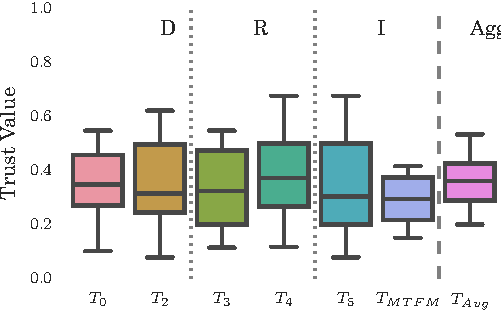
\includegraphics[width=\linewidth]{trust_bella_static_fair} 
	\label{fig:trust_static}
	\end{subfigure}%
	\begin{subfigure}{0.5\textwidth}
	\caption{Fair Mobile}
	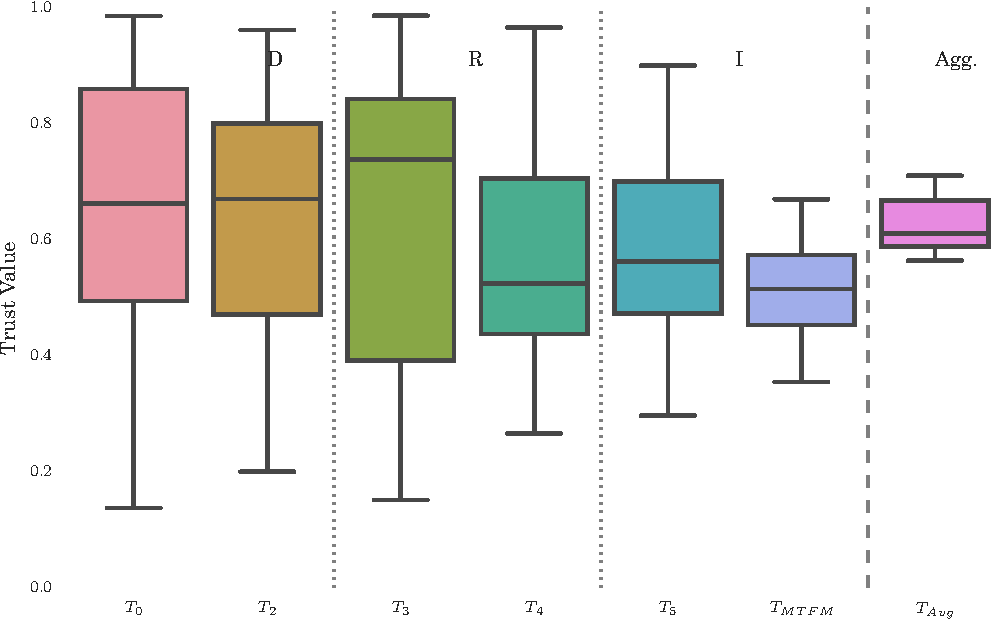
\includegraphics[width=\linewidth]{trust_bella_all_mobile_fair}  
	\label{fig:trust_all_mobile}
	\end{subfigure}%
	
	\begin{subfigure}{0.5\textwidth}
	\caption{Malicious (MPC) Static}
	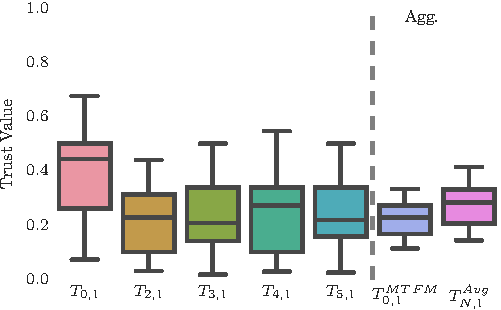
\includegraphics[width=\linewidth]{trust_bella_static_malicious} 
	\label{fig:trust_static_mal}
	\end{subfigure}%
	\begin{subfigure}{0.5\textwidth}
	\caption{Malicious (MPC) Mobile}
	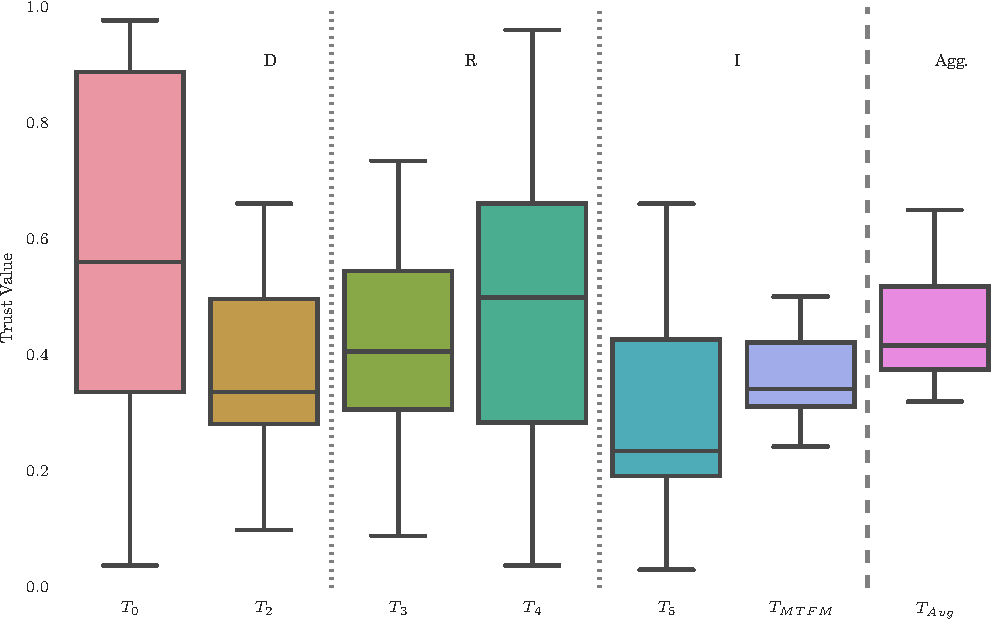
\includegraphics[width=\linewidth]{trust_bella_all_mobile_malicious}  
	\label{fig:trust_all_mobile_mal}
	\end{subfigure}%
	
	\begin{subfigure}{0.5\textwidth}
	\caption{Selfish (STS) Static}
	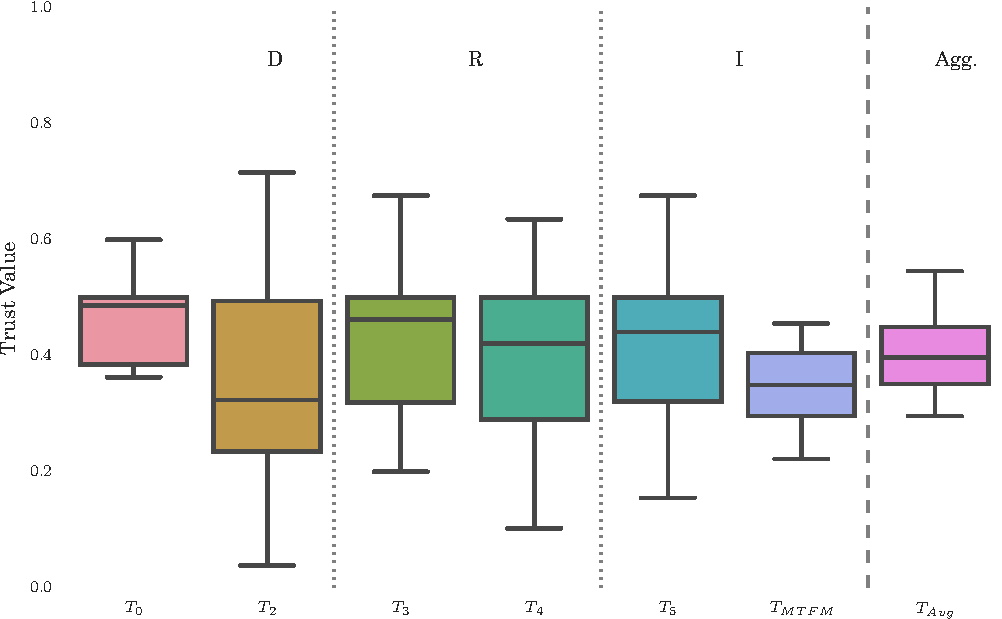
\includegraphics[width=\linewidth]{trust_bella_static_selfish}
	\label{fig:trust_static_sel}
	\end{subfigure}%
	\begin{subfigure}{0.5\textwidth}
	\caption{Selfish (STS) Mobile}
	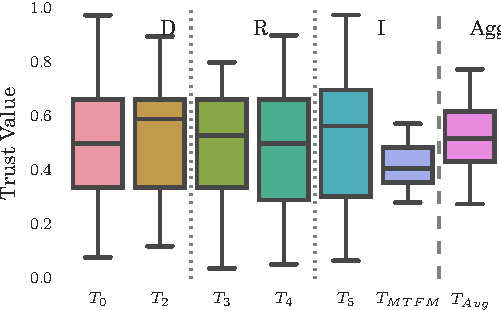
\includegraphics[width=\linewidth]{trust_bella_all_mobile_selfish}  \label{fig:trust_all_mobile_sel}
	\end{subfigure}%

	\caption{\gls{mtfm} Trust assessments of $n_1$ ($T_{1,X}$), showing Direct, Recommender and Indirect relationships, as well as the Aggregate trust assessments from combining these} 
	\label{fig:trust_mobility}
\end{figure}
%

\subsection{Comparison between \gls{mtfm}, Hermes and \gls{otmf}}
As per \cite{Guo11}, ``fair'' scenarios were also performed with no malicious behaviour, applying \gls{otmf} and Hermes assessment as well as \gls{mtfm}, providing like-for-like comparison of assessment.
For simplicity of presentation, only the fully-mobile scenario is considered, as we are concerned with the establishment of trust in mobile networks.\todo{In the thesis, we're concerned about a lot more than just the all mobile results}

\begin{figure*}[t]
  \centering
  \begin{tabular}{cc}
  \multirow{2}{*}{
  \begin{subfigure}{0.5\textwidth}	
    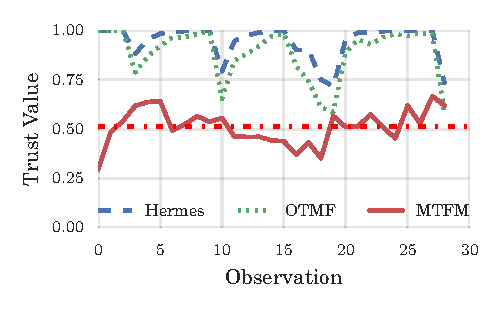
\includegraphics[width=\linewidth]{trust_beta_otmf_fair}
    \caption{Fair Scenario}
    \label{fig:all_mobile_fair_beta}
  \end{subfigure}
  }&
  \begin{subfigure}{0.5\textwidth}
    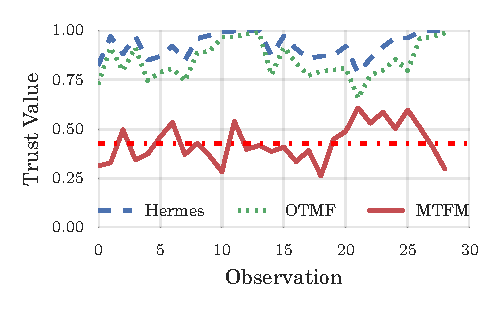
\includegraphics[width=\linewidth]{trust_beta_otmf_malicious} 
    \caption{Malicious Power Control (MPC) Scenario}
    \label{fig:all_mobile_badmouthing_beta}
  \end{subfigure} \\
  &
  \begin{subfigure}{0.5\textwidth}	
    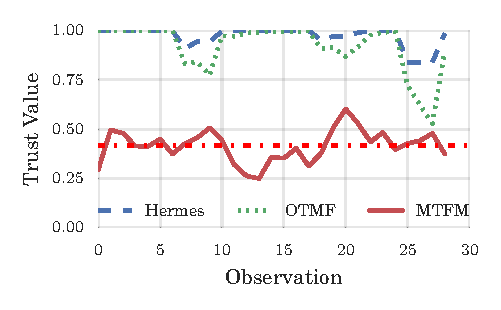
\includegraphics[width=\linewidth]{trust_beta_otmf_selfish} 
    \caption{Selfish Target Selection (STS) Scenario}
    \label{fig:all_mobile_selfish_beta}
  \end{subfigure}
\end{tabular}
  \caption{$T_{1,0}$ for Hermes, \gls{otmf} and \gls{mtfm} assessment values for fair and malicious behaviours in the fully mobile scenario (mean of \gls{mtfm} also shown)}
  \label{fig:otmf_beta_comparison}
\end{figure*}
%
The use of Forward Beam Routing and a CSMA/CA MAC scheme from AUVNetSim \cite{Miquel2008} in our simulation mitigates a significant number of packet losses through collision avoidance and contention handling, leading to the situation that the only genuinely lost packets occur when a node moves completely out of range of any other node and time out occurs in route discovery rather than transmission.
As such, confirmed packet losses are relatively rare and in a delaying network like this, it is difficult to set a differentiating time out between packets that are in the network but queued, and packets that are actually ``lost''.

The single metric \glspl{tmf} used in conventional \gls{manet}s require regular and constant input to shape and adjust their evaluations, which for a network with significant and irregular delays such as this, is not practical.
This renders \gls{otmf} and Hermes assessment at best uninformative and at worst misleading; consistently providing nodes a high trust assessment as they have very little information to extract trust from. 

Fig.~\ref{fig:otmf_beta_comparison} shows a comparison between the unweighted response of \gls{mtfm} compared to \gls{otmf} and Hermes assessment functions on the same data for the fair, malicious and selfish behaviours respectively.
It is important to note a distinction between the expectations of \gls{mtfm} compared to other \glspl{tmf}; \gls{mtfm} is primarily concerned with the identification of differences in the behaviours of nodes in a network, and is relative rather than absolute.
That is to say that under \gls{mtfm}, nodes are compared against the worst current performances across metrics of other observed nodes and graded against them, rather than the absolute (objective) approach taken by many \glspl{tmf}.
In these cases, particularly since the methods of attack were not directly related to \gls{plr}, \gls{otmf} and Hermes have not registered significant activity in either misbehaviour when compared to the fair scenario.
The difference between the \gls{mtfm} trust assessments under ``fair'' and ``malicious'' behaviour is lowered by $\approx 10\%$ in both cases, in terms of the mean values returned.
At run time, similar results could be attained by an exponentially weighted moving average filter (EWMA).

On their own, neither \gls{otmf}, Hermes, or unbiased \gls{mtfm} appear to be effective in detecting or identifying malicious behaviour in this environment, in fact \gls{otmf} and Hermes don't appear to differentiate between fair and selfish scenarios at all.


\subsection{Metric Weighting}
%

We apply a sequence of vectors that preferentially weight each metric in Eq. \eqref{eq:metric_weighting} to each of the three simulation runs.
For a metric weight vector $H$, where the metric $m_j$ is emphasised as being twice as important as the other metrics, forming an initial weighting vector $H'=[h_i\dots h_M]$ such that $h_i = 1 \forall i \ne j; h_j=2$.
We then scale that vector $H'$ such that $\sum H = 1$ by $H= \frac{H'}{\sum H'}$.
Using this process the primary aspects of an attack can be extracted and highlighted by comparing against the deviation from the ``fair'' result set. 

\begin{figure}[h]
	\centering
	\begin{subfigure}{0.45\textwidth}
		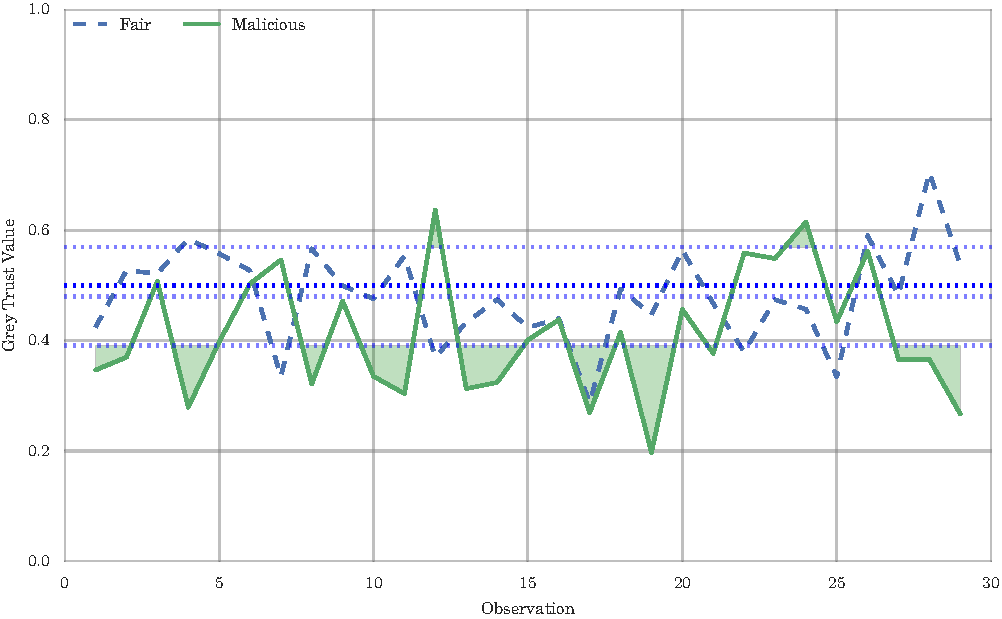
\includegraphics[width=\linewidth]{trust_bella_all_mobile_emph_ADelay_BadMouthingPowerControl} 
		\caption{Delay Emphasised}
    \label{fig:all_mobile_badmouthing_delay}
	\end{subfigure}
	\begin{subfigure}{0.45\textwidth}
		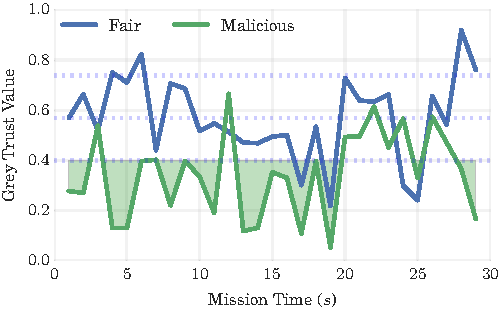
\includegraphics[width=\linewidth]{trust_bella_all_mobile_emph_PLR_BadMouthingPowerControl} 
		\caption{PLR Emphasised}
    \label{fig:all_mobile_badmouthing_plr}
	\end{subfigure}
	
	\begin{subfigure}{0.45\textwidth}
		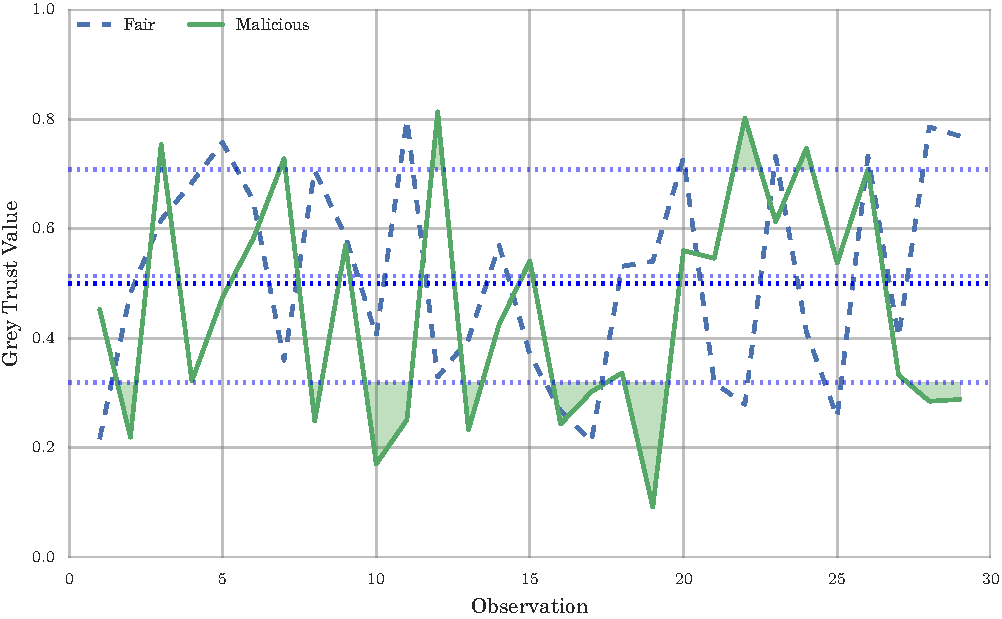
\includegraphics[width=\linewidth]{trust_bella_all_mobile_emph_ARXP_BadMouthingPowerControl} 
		\caption{RX Power Emphasised}
    \label{fig:all_mobile_badmouthing_rxp}
	\end{subfigure}	
	\begin{subfigure}{0.45\textwidth}
		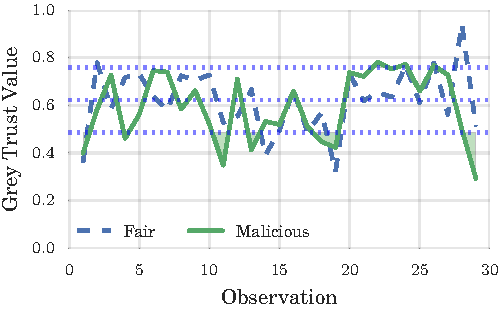
\includegraphics[width=\linewidth]{trust_bella_all_mobile_emph_ATXP_BadMouthingPowerControl} 
		\caption{TX Power Emphasised}
    \label{fig:all_mobile_badmouthing_txp}
	\end{subfigure}
	
	\begin{subfigure}{0.45\textwidth}
		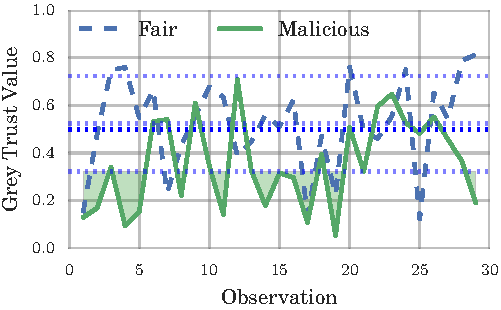
\includegraphics[width=\linewidth]{trust_bella_all_mobile_emph_RXThroughput_BadMouthingPowerControl} 
		\caption{RX Throughput Emphasised}
    \label{fig:all_mobile_badmouthing_rxthroughput}
	\end{subfigure}
	\begin{subfigure}{0.45\textwidth}
		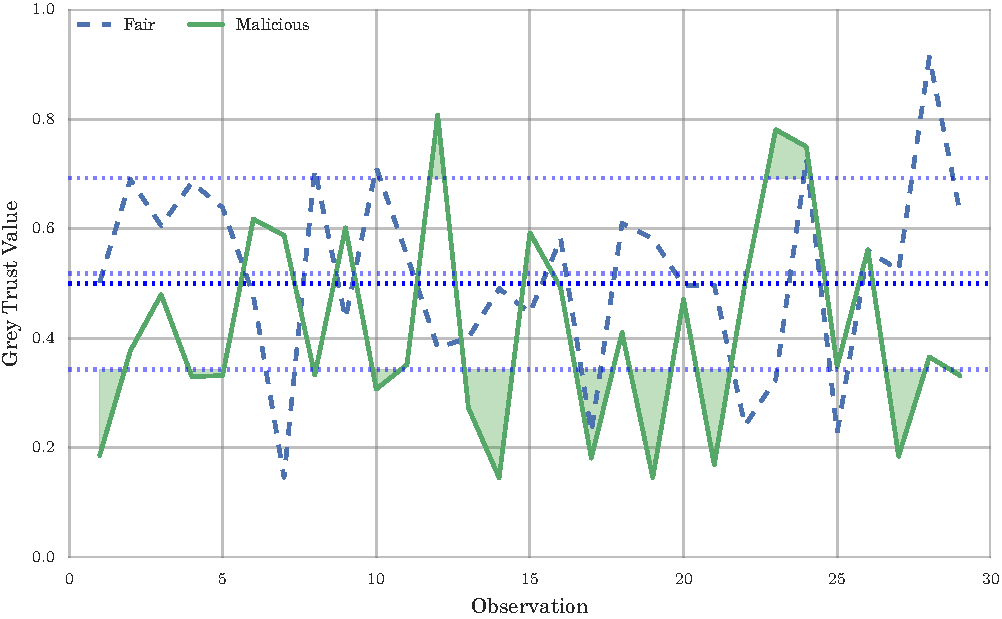
\includegraphics[width=\linewidth]{trust_bella_all_mobile_emph_TXThroughput_BadMouthingPowerControl} 
		\caption{TX Throughput Emphasised}
    \label{fig:all_mobile_badmouthing_txthroughput}
	\end{subfigure}
	\caption{$T_{1,MTFM}$ in the All Mobile case for the Malicious Power Control behaviour, including dashed $\pm\sigma$ envelope about the fair scenario}
	\label{fig:all_mobile_badmouthing}
\end{figure}
%
\begin{figure}[h]
  \centering
  \begin{subfigure}{0.45\textwidth}	
    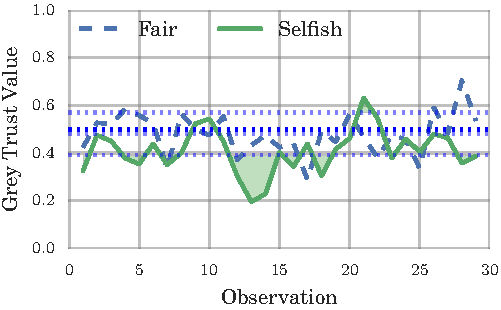
\includegraphics[width=\linewidth]{trust_bella_all_mobile_emph_ADelay_SelfishTargetSelection} 
    \caption{Delay Emphasised}
    \label{fig:all_mobile_selfish_delay}
  \end{subfigure}
  \begin{subfigure}{0.45\textwidth}	
    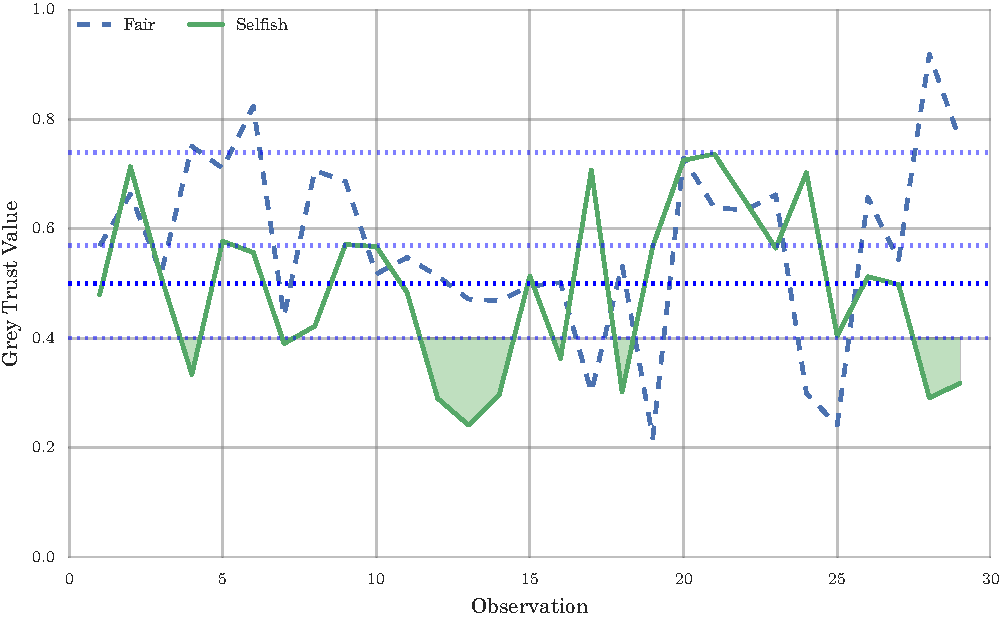
\includegraphics[width=\linewidth]{trust_bella_all_mobile_emph_PLR_SelfishTargetSelection}
    \caption{PLR Emphasised}
    \label{fig:all_mobile_selfish_plr}
  \end{subfigure}

  \begin{subfigure}{0.45\textwidth}	
    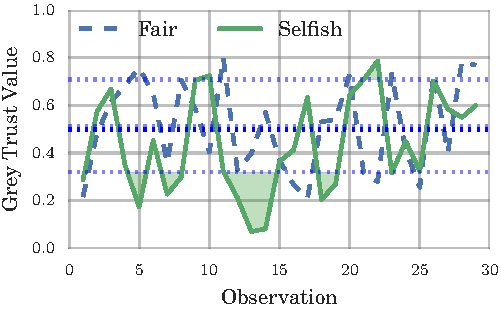
\includegraphics[width=\linewidth]{trust_bella_all_mobile_emph_ARXP_SelfishTargetSelection}
    \caption{RX Power Emphasised}
    \label{fig:all_mobile_selfish_rxp}
  \end{subfigure}
  \begin{subfigure}{0.45\textwidth}
    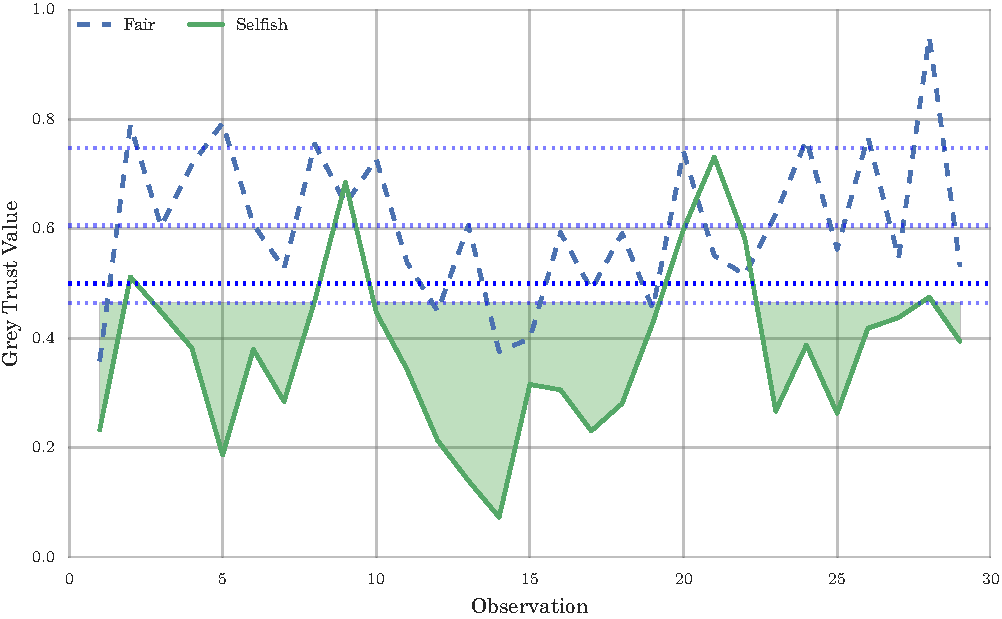
\includegraphics[width=\linewidth]{trust_bella_all_mobile_emph_ATXP_SelfishTargetSelection}
    \caption{TX Power Emphasised}
    \label{fig:all_mobile_selfish_txp}
  \end{subfigure}

  \begin{subfigure}{0.45\textwidth}
    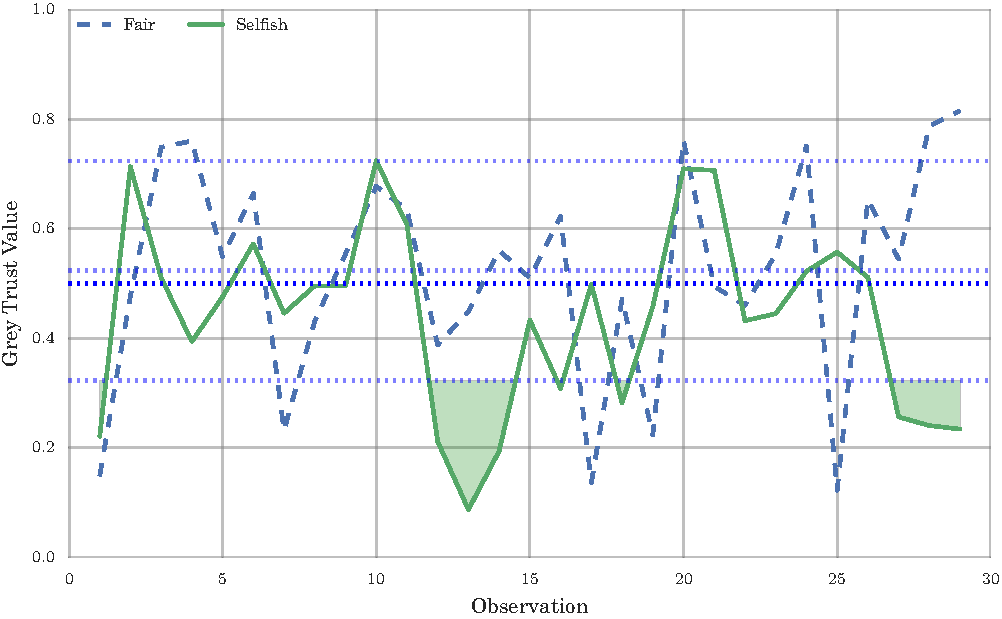
\includegraphics[width=\linewidth]{trust_bella_all_mobile_emph_RXThroughput_SelfishTargetSelection} 
    \caption{RX Throughput Emphasised}
    \label{fig:all_mobile_selfish_rxthroughput}
  \end{subfigure}
  \begin{subfigure}{0.45\textwidth}
    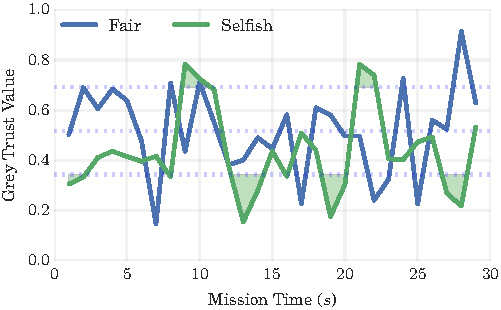
\includegraphics[width=\linewidth]{trust_bella_all_mobile_emph_TXThroughput_SelfishTargetSelection} 
    \caption{TX Throughput Emphasised}
    \label{fig:all_mobile_selfish_txthroughput}
  \end{subfigure}
  \caption{$T_{1,MTFM}$ in the All Mobile case for the Selfish Target Selection behaviour, including dashed $\pm\sigma$ envelope about the fair scenario}
  \label{fig:all_mobile_selfish}
\end{figure}

Fig.~\ref{fig:all_mobile_badmouthing} shows that the malicious node is consistently outside the $\pm\sigma$ (one standard deviation above and below the mean) envelope of the fair scenario it's being compared to.
This is particularly true for \gls{plr}, with smaller impacts on delay, received power and transmitted throughput. 
This weighted delta in received throughput is minimal to insignificant compared to the width of the detection envelope, occasionally breaching the envelope for a short period. 

In the selfish case (Fig.~\ref{fig:all_mobile_selfish}) a much lower weighted delta in \gls{plr} and delay is observed, with greatly increased impact on transmission power.
In comparison to \cite{Guo11}, these results are qualitatively similar, however here the differences between the fair case and the misbehaviours are less clear than in the comparable terrestrial space.
Guo et al.\ show similar types of behaviour but report a weighted delta from $\approx$ 0.4 to $\approx$ 0.9 across the simulation period, compared to our maximum delta in $P_{TX}$ in selfish behaviour (Fig.~\ref{fig:all_mobile_selfish_txp}) of $\approx$ 0.3 for an inconsistent interval.


\subsection{Weight Significance Analysis for Behaviour Classification}

For a more quantitative assessment of the viability of multi-metric trust assessment methods, taking the qualitative analysis above and apply a Random Forest regression \cite{Breiman2001} to assess the relative importance of the selected metrics on relative detectability of malicious behaviour. 
Random Forest accomplishes this by generating a large number of random regression trees and prune these trees to fit incoming data.
The target function for this regression was the area between the target behaviours weighted $T_{MTFM}$ curve and the $\pm\sigma$ envelope of the base behaviour as shaded in Figs.~\ref{fig:all_mobile_badmouthing} and~\ref{fig:all_mobile_selfish}.
From this training process, the relative importance of each input feature (metric) can be inferred in terms of how good it is to differentiate between the fair case and a given misbehaviour.
Additionally a cross correlation analysis is performed to establish the correlations between given metric weighting emphasis and the output of the target function.
Our intention is to establish the metrics that not only differentiate both misbehaviours from the fair case, but also what metrics differentiate the two misbehaviours from each other.

Applying this target regression to 729 different metric weight vector emphasis combinations reveals that each of the three combinations (i.e.\ comparing fair to misbehaviours, and comparing the misbehaviours) present distinct patterns of significance in three primary metrics; received throughput, transmitted power, and PLR, with delay, received power and transmitted throughput playing a lesser role.
Practically this means that in order to accurately distinguish between these scenarios, these primary metrics should be higher-weighted in the generation of $T_{1,MTFM}$ in \eqref{eq:networkeffects}.

It may initially appear odd that the relative significance of the received throughput is similar between all three scenario combinations, however a correlation analysis shows that in the MPC attack; the received throughput is positively correlated with successful classification against the fair case ($R=+0.71, p\approx10^{-100}$), while the inverse is the case for the STS attack ($R=-0.70, p\approx10^{-100}$).
It is expected that Transmitted power should be the defining characteristic of STS ($R=+0.72, p<10^{-100}$) as the node is acting fairly from a protocol perspective but is acting unfairly at a higher (incentive) level; it is performing fairly in terms of it's communications with other nodes, however it is preferring to communicate with nodes that it can expend less energy communicating with.
A summary of these correlations is shown in Table.~\ref{tab:correlations}.

Comparing Figs.~\ref{fig:otmf_beta_comparison},~\ref{fig:all_mobile_badmouthing_plr}, and~\ref{fig:all_mobile_selfish_plr}, while it is possible that in a cleaner, less sparse, and less noisy environment, \gls{otmf} would be able to detect the \gls{mpc} behaviour, Fig.~\ref{fig:malselfactors} shows that \gls{plr} plays almost no part at all in detecting the \gls{sts} behaviour, and so \gls{otmf} would not detect the attack.

\begin{figure}
	\centering
	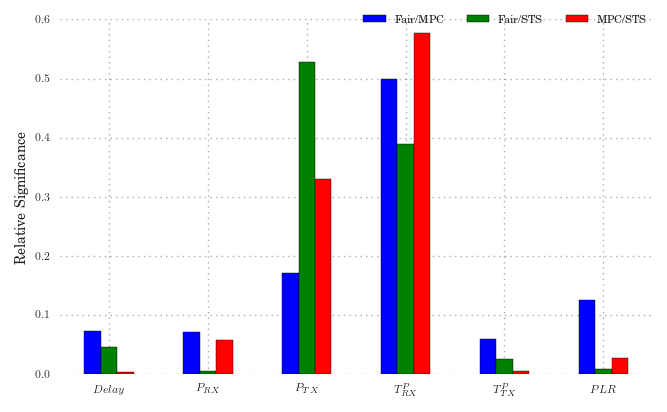
\includegraphics[width=0.95\linewidth]{MaliciousSelfishMetricFactors}
	\caption{Random Forest Factor Analysis of Malicious (\gls{mpc}, Selfish (\gls{sts}) and Fair behaviours compared against each-other}
	\label{fig:malselfactors}
\end{figure}

\begin{table}[h]
	\caption{Correlation Coefficients between metric weights and behaviour detection targets} \label{tab:correlations}
	\begin{center}
		\begin{tabular}{lcccccc}
			\toprule
			Correlation      & Delay & $P_{RX}$ & $P_{TX}$ & $T^P_{RX}$ & $T^P_{TX}$ & PLR \\
			\midrule
			Fair / MPC       & 0.199 &  0.159   & -0.416  &  0.708   & -0.238   & -0.401\\
			Fair / STS       & 0.179 &  -0.009  &  0.724  & -0.697   & -0.145   & -0.052\\
			MPC / STS        & 0.058 &  -0.134  &  0.146  & -0.768   &  0.052   &  0.146\\
			\bottomrule
		\end{tabular}
	\end{center}
\end{table}

As such this presents the open opportunity to develop a heuristic weight search scheme to detect malicious behaviour without the comparison to the fair scenario.
This would be accomplished by assessing the impact of differential metric weighting on the mean trust assessment rather than comparing co-weighted valuations across scenarios.


\section{Conclusions and Future Work}
We have demonstrated that existing \gls{manet} Trust Management Frameworks are not directly suitable to the sparse, noisy, and dynamic underwater medium.
We presented a comparison between trust establishment in \gls{manet}s in a simulated underwater environment, demonstrating that in order to have any reasonable expectation of performance, throughput and delay responses must be characterised before implementing trust in such environments. 
While the \gls{mtfm} value does not display any immediate difference between the two behaviours, it has been shown that by exploring the metric space by weight variation, the existence and nature of the malicious behaviour can be discovered.
Another difference is that \gls{mtfm} is significantly more computationally intensive than the relatively simple Hermes / \gls{otmf} algorthms.
The repeated metric re-weighting required for real time behaviour detection is therefore an area that requires optimization.
We demonstrated initial, unfiltered Grey Trust assessment using all available metrics (transmitted and received throughput, delay, received signal strength, transmitted power, and packet loss rate), as well as the application of multiple weighting vectors to iteratively emphasise different aspects of trust operation to expose and identify misbehaviour on the network.
With significant delays (from seconds to many minutes), in a fading, refractive medium with varying propagation characteristics, the environment is not as predictable or performant as classical \gls{manet} \gls{tmf} deployment environments.

We show that, without significant adaptation, single metric probabilistic estimation based \glspl{tmf} are ineffective in such an environment.
We have shown that existing frameworks are overly optimistic about the nature and stability of the communications channel, and can overlook characteristics that are useful for assessing the behaviour of nodes in the network. 
This indicates that there is a good case, particularly within constrained \gls{manet}Ìs as this, for multi-vector, and even multi-domain trust assessment, where metrics about the communications network and topology would be brought together with information about the physical behaviours and operations of nodes to assess trust.

Also, a significant factor of trust assessment in such a constrained environment, is that there may be long periods where two edge nodes (for instance, $n_0 \to n_5$) may not interact at all. 
This can be due to a range of factors beyond malicious behaviour, including simple random scheduling coincidence and intermediate or neighbouring nodes collectively causing long back-off or contention periods.
This disconnection hinders trust assessment in two ways; assessing nodes that do not receive timely recommendations may make decisions based on very old data, and malicious nodes have a long dwelling time where they can operate under a reasonable certainty that the \gls{tmf} will not detect it (especially if the node itself is behaving disruptively).
One solution to this would be to move from a stepping-window of trust observations to a continuous trust log, updated on packet reception rather than waiting regular periods for packets to be analysed.
Future work will investigate the improvement of weight-based detection algorithms, the stability of GRA under multi-node collusion, the development of real-time outlier detection, and the introduction of physical behavioural metrics into the trust assessment context.





%%%%%%%%%%%%%%%%%%%%%%%%%%%%%%%%%%%%%%%%%%%%%%%%%%%%%%%%%%%%%%%%%%%%%%%%%%%%%%%
\ifx\ifthesis\undefined
	%% ----------------------------------------------------------------
\label{Bibliography}
% \bibliographystyle{amsplain}
%\bibliographystyle{unsrtnat}  % Use the "unsrtnat" BibTeX style for formatting the Bibliography
\bibliographystyle{alpha}
\bibliography{../Thesis}  % The references (bibliography) information are stored in the file named "Thesis.bib"

\end{document}  % The End
%% ----------------------------------------------------------------
\else
\fi
